\chapter{Background}

%\newcommand{dltext}[1]{\centerline{\textsf{#1}\newline}}

\section{Knowledge Graphs}
There is no single agreed upon definition of \glspl{kg} \cite{bergman_2019, bonatti2019knowledge, ehrlinger2016towards}. Definitions and usages vary from specific technical proposals to more general descriptions. In this thesis we will use the more inclusive definition similar to the one proposed by Hogan et al. \cite{hogan2020knowledge}, where we view a \gls{kg} as \textit{a graph of data intended to capture the semantic connections within real world knowledge, where nodes represent relevant entities and edges represent relations between these entities}. The type of graph may vary, i.e. it may be simple, directed, etc. A graph may contain knowledge over a broad range of domains, such as Wikidata\cite{lehmann2015dbpedia}, or be limited to a specific domain, such as DBpedia\cite{fellbaum2010wordnet}. The concept of ``knowledge'' has been widely debated in epistemology, but here we will use it to mean descriptive knowledge, meaning facts that can be stated. Knowledge can be simple statements, such as ``Leo is a cat'', or quantified statements such as ``at least one cat is black''. KGs are not expressive enough for quantified statements, where ontologies or rules would be more appropriate. Additional knowledge can be inferred from KGs through inductive or deductive methods. For example from a KG containing the information that ``Leo is a cat'' and ``cats are mammals'', one can deductively infer that ``Leo is a mammal''. If all cats mentioned in the knowledge graph like to eat fish, then one can inductively infer ``cats like to eat fish''.


%For example, the knowledge that 'Amy is the daughter of Bo, and Bo is a woman' can be represented by the knowledge graph in fig 1.\todo{Add figure}
\begin{figure}[h]
\centering
\begin{tikzpicture}
    \node[shape=circle,draw=red] (L) at (0,0) {Leo};
    \node[shape=circle,draw=black] (C) at (3,0) {Cat};
    \node[shape=circle,draw=black] (M) at (1.5,3) {Mammal};

   % \path [->] (L) edge node[left] {$IsA$} (C);
   \draw [->] (L) -- (C);
   \draw [decoration={text along path,
    text={is a},text align={center}},decorate]  (L) -- (C);
    
    \draw [->] (C) -- (M);
   \draw [decoration={text along path,
    text={subclass},text align={center}},decorate]  (M) -- (C);
    
    \draw [dotted, ->] (L) -- (M);
   \draw [decoration={text along path,
    text={is a},text align={center}},decorate]  (L) -- (M);
    
\end{tikzpicture}

\caption{Example of a knowledge graph, where the dotted line represents a relationship that can be deductively inferred.} \label{fig:KGexample}
\end{figure}

In this thesis we will loosely follow the Resource Description Framework (RDF) standard and view KGs as sets of semantic triples. RDF is a standard for representation and exchange of graph data introduced by \gls{w3c}. Semantic triples are the data types used in the RDF data model. A triple, as the name suggests, is a tuple of three elements. It has the form ( subject, predicate, object) and can therefore represent statements about semantic data, for example "Cats are mammals", or "Ann knows Bob". These RDF statements express relationships between two resources, these resources being the subject and the object, while the predicate encapsulates the nature of the relationship. The relationship is phrased in a directional way, and so set of RDF stamements can also be viewed as a directed graph. The graph represents these triple statements, where the predicate in the triple denotes the edge going from the subject to the object, both of which are vertices.

\begin{lstlisting}[caption={Example of RDF triple set written in informal pseudocode},label={RDF_triples_example}][h]
<Leo> <is a> <cat>
<cat> <is a> <mammal>
<Ann> <knows> <Bob>
<Ann> <is a> <person>
<Bob> <is a> <person>
<Ann> <has pet> <Leo>
\end{lstlisting}

%For example, the knowledge that 'Amy is the daughter of Bo, and Bo is a woman' can be represented by the knowledge graph in fig 1.\todo{Add figure}
\begin{figure}[h]
\centering
\begin{tikzpicture}
    \node[shape=circle,draw=black] (L) at (3.9,0) {Leo};
    \node[shape=circle,draw=black] (P) at (0,2.5) {Person};
    \node[shape=circle,draw=black] (A) at (1,0) {Ann};
    \node[shape=circle,draw=black] (B) at (2.5,2.5) {Bob};
    \node[shape=circle,draw=black] (C) at (6,0) {Cat};
    \node[shape=circle,draw=black] (M) at (5,2.5) {Mammal};

   % \path [->] (L) edge node[left] {$IsA$} (C);
   \draw [->] (L) -- (C);
   \draw [decoration={text along path,
    text={is a},text align={center}},decorate]  (L) -- (C);
    
    \draw [->] (L) -- (M);
   \draw [decoration={text along path,
    text={is a},text align={center}},decorate]  (L) -- (M);
    
    \draw [->] (A) -- (B);
   \draw [decoration={text along path,
    text={knows},text align={center}},decorate]  (A) -- (B);
    
    \draw [->] (A) -- (L);
   \draw [decoration={text along path,
    text={has pet},text align={center}},decorate]  (A) -- (L);
    
    \draw [->] (A) -- (P);
   \draw [decoration={text along path,
    text={is a},text align={center}, reverse path},decorate]  (A) -- (P);
    
    \draw [->] (B) -- (P);
   \draw [decoration={text along path,
    text={is a},text align={center}, reverse path},decorate]  (B) -- (P);
    
\end{tikzpicture}

\caption{Informal visualization of the KG consisting of the example triples from \ref{RDF_triples_example}} \label{fig:KGexample}
\end{figure}

With this type of data organisation one can for example query for a list of all people who own cats in the dataset.

\subsection{Integrity of KGs}
\label{Integrity_of_KGs}
Amihai Motro presents in his paper 
KGs contain only true facts. By the \textit{closed world assumption } (CWA) all facts not present in the KG are considered false. For example, by the KG in figure \ref{fig:KGexample} the statement \texttt{<Ann> <has sibling> <Bob>} is false under the CWA, as it is not present in the KG. Bob is not the sibling of Ann. The \textit{open world assumption} (OWA) makes no such claims and  the validity of a triple not present in the KG is considered unknown. In the above example Bob is therefore neither considered a sibling of Ann nor not a sibling of Ann.

In the context of KGs the OWA is often more justified, as most large interesting KGs are far from complete. For example, the KG Wikidata5M does not contain about information the national bird of countries. This of course does not make the statement ``\textit{The kiwi is the national bird of New Zealand}" any less true. The information has simply not been included in the KG. Another example is Freebase, the precursor to Wikidata, in which 71\% is people listed had the place-of-birth attribute missing.

\begin{figure}[htp]
    \centering
    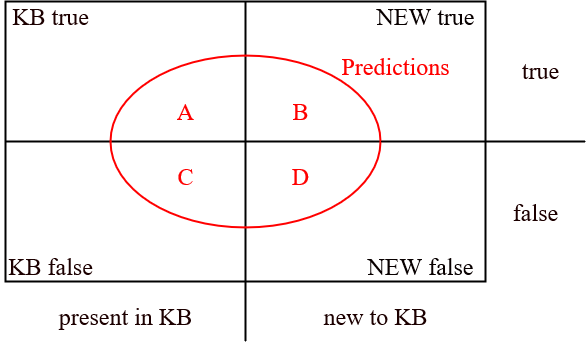
\includegraphics[width=10cm]{figures/kb_venn.png}
    \caption{KB prediction under incompleteness}
    \label{KB_predictions}
\end{figure}

However, in the context of rule mining and KG embeddings the OWA has a central problem; it fails to provide counterexamples. Because missing facts are assumed to be neither true nor false, there are no false facts to give as examples when mining rules or training an embedding model. In the context of the predictions, marked with red in \cref{KB_predictions} we want to maximize B over D. Under the OWA, however, there are no false facts, so we don't know what B and D are. The authors of AMIE therefore introduced a new paradigm called the \textit{partial completeness assumption} (PCA). It assumes that if $r(x, y) \in KB true$ for some entities $x$, $y$, then
\[\forall y' : r(x, y') \in KBtrue \cup NEWtrue \Rightarrow r(x, y') \in KBtrue\].
This assumption says that if the KG already has $r$-related information about the entity $x$,  then it contains \textit{all} $r$-related information about $x$. For example if a KG only contains \texttt{<Ann> <has sibling> <Bob>} and no other sibling entries with Ann as the head, then by the PCA Bob is Ann's only sibling. All other facts claiming that Ann has other siblings will therefore be negative examples. If we then however ask what \textit{friends} Ann has in a knowledge base without information about Ann's friends, then one cannot conclude that Ann is friendless. PCA is a more particular version of the broad \textit{partial-closed world assumption} (PCWA), where the KG generally is treated under the OWA, but parts of it that are considered complete are treated under the CWA \cite{motro1989integrity}. The PCA specifically defines what parts of the KG should be treated under closed-world semantics.



\section{Knowledge Graph Embeddings}
Let $\mathcal{K}$ be a KG with triples of the form $<h, r, t>$ with $r\in \mathbb{R}$ and $h, t \in \mathbb{E}$, where $\mathbb{R}$ and $\mathbb{E}$ are respectively the set of all relations and entities in $\mathcal{K}$. To simplify the explanation we let the dimension of entities \emph{and} relations in the embedding space to be $d$.
Given $\mathcal{K}$ and $d$, a KG embedding seeks to represent all entities and relations in the continuous vector space of $d$ dimensions. These representations are meant to capture the semantic information in the graph. An embedding that manages this can then be used to evaluate the probability of new facts and identify false information in $\mathcal{K}$, two tasks respectively called \textit{link prediction} and \textit{triple classification}. Let $\text{\textbf{(h, r, t)}}$ denote an embedding of a head, relation and tail. 

The procedure for training KG embedding models is similar to any other statistical-based machine learning. The values of the embeddings are usually initialized as random values. These embeddings are continuously optimized through a training loop, which stops once the stop condition is met (usually overfitting on the training set). For each triple in the training set, $\eta$ negative counterexamples are generated by triple corruption. This is done by swapping out either the head $h$ or (not both) tail $t$ with some other $h', t' \in \mathbb{E}$ \cite{TransE}. Both the original triple and the corrupted triples are added to the training batch. A \textit{scoring function} is used to measure the "goodness" or plausibility of a triple. The model should give a good score to triples from the KG, and a bad score to the corrupted triples. By updating the embedding to optimize the scoring function the model should at the end of training have meaningful embeddings that can accurately evaluate unseen triples. In the training process this is done by minimizing the model's \textit{loss function}.

\subsection{Loss functions}
A loss function is a function that assigns a cost to an event in the form of a real number. Optimization algorithms aim to minimise the loss function. In the context of KG embedding models many different types of loss functions can be used. 

This goes pretty in depth: https://ieeexplore.ieee.org/stamp/stamp.jsp?tp=&arnumber=9416312


Loss functions:
    - Pairwise
    - Negative log loss likelyhood (nll)
    
    
    
    
\subsection{ComplEx}
ComplEx is a tensor factorization-based embedding model.\nocite{trouillon2016complex} In such models triples in a KG are transformed into a 3D binary tensor. The embeddings of the entities and relations are intended to be such that one can mathematically combine them to obtain the tensor representing the KG. ComplEx builds on the embedding model DistMult, which restricts the semantic embedding of relations to be a diagonal matrix. This allows for the number of parameters to be linear on the number of entities and embedding dimension. \nocite{dai2020survey} 

Unfortunately the original DistMult model cannot embed asymmetric relations, which the ComplEx approach solved by using complex-valued embeddings. This was achieved without increasing parameter or memory complexity. The imaginary and real part of the embeddings play the role of representing the "direction" of the relation and thus asymmetric relations are able to be embedded. I used \href{https://docs.ampligraph.org/en/1.4.0/generated/ampligraph.latent_features.ComplEx.html}{Ampligraph's} implementation of ComplEx, but it provided to be problematic to use. Explanation of the problems encountered are described in the \textbf{Experiments} section.    
    



\textbf{Metrics}

    Ranking triples
    
\subsection{Performance indicators}

    MR

    MRR

    Hits@n
    


\section{Rule-based machine learning}
Rule-based machine learning has as a goal to create rules that make new true predictions going beyond the data on which the rule was applied to. In contrast, other areas of machine learning focus on training a single model that can be applied to make a broad range of predictions. Conceptually the end result of rule-based machine learning is similar to a rule-based system.  Rule-based systems are often hand-crafted and require a knowledge expert to be curated, while rule-based machine learning requires no knowledge expert and rules are automatically created by the learning algorithm.

Classically, a rule is comprised of a condition and consequent, or a so-called "if-then" statement. \begin{center} \textbf{IF} \textit{'the condition is met'} \textbf{THEN} \textit{'the consequent holds'} \end{center}
The condition of the rule specifies attributes in the data on which the rule will be applied. If these attributes are present in this data, the condition is met. Once the condition for the rule is met, the attributes in the consequent should necessarily also be met. We define an \textit{atom} to be a triple in which the head and/or tail are variables. A \textit{Horn rule} is a rule where the consequent of a rule is a single atom, while the body is a set of atoms. We denote a Horn rule by $B \Rightarrow r(x, y)$ where $B$ is the body and $r(x, y)$ the head. Two examples of such rules are \ref{example_rule_1} and \ref{example_rule_2}.

\begin{equation}
hasSibling(x, y) \Rightarrow hasSibling(y,x)
\label{example_rule_1}
\end{equation}
\begin{equation}
    hasSibling(x, y), hasMother(y,z) \Rightarrow hasMother(x,z)
    \label{example_rule_2}
\end{equation}
\begin{lstlisting}[caption={Simple example knowledge base},captionpos=b, label={simple_kb_example}]
<Ann> <hasMother> <Carol>
<Ann> <hasSibling> <Bob>
<Bob> <hasSibling> <Ann>
\end{lstlisting}
Consider the two rules and knowledge base given above. Under this knowledge base the antecedent of the first rule is satisfied by both triple 2 and 3. The resulting consequent of rule \ref{example_rule_1} is also present in the knowledge base. So the reflexivity of the $hasSibling$ predicate holds in this knowledge base. The antecendent of the second rule is satisfied by triples 1 and 2 in the knowledge base, but the resulting consquent would then be $hasMother(Bob, Carol)$. Since \texttt{<BoB> <hasMother> <Carol>} is not present in the knowledge base, rule \ref{example_rule_2} does not hold. If we know that this rule is reliable, we could for example extend the incomplete knowledge base with this triple.

Within rule-based machine learning there are many different approaches including learning classifier systems \cite{sigaud2007learning} and association rule mining \cite{agrawal1993mining}, the latter of which is the approach used in this thesis. Both approaches aim to create a set of rules to act as a model for a set of data. The association rule mining approach will now be explained further.


\subsection{Association Rule Mining}
Association rules \cite{agrawal1993mining} are types of "if-then" statements that describe frequent associations between items in a dataset containing \textit{transactions}. Association rule mining was originally proposed as a new method for finding relationships between sales items in stores. The idea of mining association rules over transactions has successfully been applied to many other scenarios \cite{altaf2017applications, lin2002efficient}. In the context of convenience store sales, each transaction can be thought of as a set of items that a customer has purchased. The rules are of the form $\{Sugar, Flour, Eggs\} \Rightarrow Butter$, meaning that a person who bought sugar, flour and eggs was likely to also purchase butter. The antecedent is some set of items in the dataset, while the consequent is an item often found in combination with the antecedent in the dataset.  So sugar, flour and eggs can be thought of as "associated with" butter. These original association rules are also not Horn rules over binary predicates, but is cited as a main inspiration for the AMIE3 approach used for experiments in this thesis. AMIE3 also limits rules to be in Horn form, meaning that the consequent can contain at most one predicate. We denote a Horn rule by $B \rightarrow r(x,y)$

\subsection{Significance and quality measurement}
The goal is to find formal rules that make true predictions that go beyond the explicit information in the knowledge base. If we look back at \cref{KB_predictions} this means we want to maximise B and minimise D. For this we need to know what those areas are, and this is where the problem of missing negative examples from \cref{Integrity_of_KGs} occurs as the area \textbf{KB false} is empty. We will look at different measures that address this problem.

\subsubsection{Support}
The \textit{support} of a rule is the quantity of correct predictions. So, if we consider \cref{KB_predictions} as a diagram representing the predictions of a rule $B \rightarrow r(x,y)$, then the support of the rule is area A. What counts as an instance of a correct prediction can very. The authors of AMIE3 point out that if one chooses the number of instantiations of the rule, then the measure becomes non-monotonic. They give an example with the rule:
\[marriedTo(x, y) \Rightarrow marriedTo(y, x)\]
where if $hasGender(x, male)$ is added to the body, then the number of instantiations in the KB can only decrease. If on the other hand $haFriend(x, z)$ is added to the body then the number of instantiations may increase. In order to preserve monoticity and only a single measure of support  for each rule they define the support of a rule to be the number of distinct object-subject pairs in the KB that appear in the head and tail of the rule:
\[supp(\vec{B}\Rightarrow r(x, y)) :=  \# (x, y) : \exists z_1 , ...,z_m : \vec{B} \wedge r(x, y)\]


\subsubsection{Head coverage}
Support is not an absolute measurement, rather a relative measurement. It requires the complete size of the KG for the values to have meaning. This is countered with a proportional version of support called \emph{head coverage}. It is the ratio of known true facts about a relation $r$ that are implied by the rule with $r$ in its head:
\[hc(B \rightarrow r(x,y)) = \frac{support(B \rightarrow r(x,y))}{|\{(x, y) : r(x, y) \in \mathcal{K}\}|}\]
We now have an absolute measurement of significance, but this is not a measure of quality of a rule, only relevance. For this we need confidence measures.


\subsubsection{Standard Confidence} Confidence is the proportion of a rules true predictions out of all its predictions. In order to determine if a new fact is true or false, one must make assumptions about the facts missing from the KG. The \textit{standard confidence} adopts the CWA and labels all facts not already present in the KG as false. Thus, the standard confidence of a rule is the ratio of its predictions that are in the KG:
\[conf(\vec{B}\Rightarrow r(x, y)) := \frac{supp(\vec{B}\Rightarrow r(x, y)}{\#(x, y):\exists z_1 ,..., z_m : \vec{B}}\]

If one wants to mine rules that only describe the data at hand, and has a relatively complete KG, then this is a good measure of confidence. If the aim on the other hand is to mine rules that predict new facts then standard confidence is not a good measurement as it penalizes rules that make predictions outside of the current knowledge.

\subsubsection{PCA Confidence}
Recalling the PCA from \ref{Integrity_of_KGs} we now look at AMIE's attempt at normalizing the confidence by identifying negative examples with the PCA. The confidence is not normalized by the entire set of facts, rather with the set of facts known to be true (those in the KG), and those assumed to be false (with PCA). Thus, the \textit{PCA confidence} is defined as:
\[pcaconf(\vec{B}\Rightarrow r(x, y)) := \frac{supp(\vec{B}\Rightarrow r(x, y)}{\#(x, y):\exists z_1 ,..., z_m, y' : \vec{B} \wedge r(x, y')}\]


\subsection{AMIE, AMIE+ and AMIE3}
\textcolor{red}{I treat the mining algorithm as a black box in the experiments. How much shoulf be written about AMIE3 here= Should I write about the different versions of AMIE?}

\iffalse 
\section{Web Ontology Language}
A widely used formal language for expressing ontologies is the \gls{owl}. In OWL "Daughters are female" could be formally expressed as:

\centerline{\textsf{SubClassOf(Daughter Female)}}
Information expressed in OWL can be used to draw new conclusions. For example if we know that an individual \emph{Amy} is a daughter, then we can makes the same conclusions as earlier about Amy being female. In OWL, the fact that Amy is in the class of females can be expressed as:

\centerline{\textsf{ClassAssertion(Female amy)}}
The task of reaching such conclusions is called reasoning and the type of conclusions that can be drawn is specified by the \gls{w3c}. It specifies the \emph{semantics} of OWL, but does not present algorithms for how to derive inferences in practice. Sound and complete reasoning in OWL is of high complexity \cite{Krotzsch2012}. Therefore, when the standard was updated to OWL 2 in 2009, it introduced restricted sublanguages to address this problem. These sublanguages restrict expressivity in order to simplify the reasoning task. One of these languages is OWL 2 QL, which is based on a \gls{dl} language called DL-Lite. OWL 2 QL is intended as a language to enable easier queries to databases. The ontology language we will use is DL-Lite$_{\mathcal{R}, horn}^{\exists}$, which is a member of the DL-Lite family.



\section{Description Logics}
\gls{dls} are a family of languages used in knowledge representation and reasoning. They are generally less expressive than \gls{fol}, but more expressive than \gls{pl}. The name \textit{description logic} represents two central aspects to this language group: \emph{description}, formal expression of knowledge, and  \emph{logic}, for it's logic-based semantics. DLs are used to represent domain knowledge in a well-structured and easily interpretable way. Domain knowledge is separated into two components in DL, a \emph{terminological} part, called a TBox, and an \emph{assertional} part, called an ABox. The TBox represents knowledge about the structure of the domain, while the ABox has knowledge about specific instances. For example the fact that \emph{cats are  mammals} would be a TBox statement, while \emph{Leo is a cat} would be an ABox statement, as here we are making an assertion about the individual Leo. The combination of a TBox and an ABox is called a \emph{knowledge base} (KB).
As the semantics of DLs are logic-based it is clear when a statement is \emph{entailed} by a KB. For instance the two examples given above entail that Leo is a mammal. More importantly, this reasoning task can be automated in a DL KB. Reasoning tasks are performed with respect to the entire KB, which gives this language great power, but also comes with a computational cost. Therefore an important area of research has been to find DLs that strike a balance between expressiveness and the computational complexity of reasoning.


The two main criteria for a reasoner is that it is decidable and tractable (always correctly completed in a time that is polynomial with respect to the size of the KB). The more operators one allows in a logic the more complicated the TBox becomes, and usually the complexity for reasoning in the language increases. See \href{http://www.cs.man.ac.uk/~ezolin/dl/}{\textbf{Complexity of reasoning in Description Logics}} for an interactive look at the complexity of different DLs \cite{zolin_2013}.

\section{The Resource Description Framework}

The Resource Description Framework (RDF) is a standard for representation and exchange of graph data introduced by \gls{w3c}. Semantic triples are the data types used in the RDF data model. A triple, as the name suggests, is a tuple of three elements. It has the form ( subject, predicate, object) and can therefore represent statements about semantic data, for example "Cats are mammals", or "Ann knows Bob". These RDF statements express relationships between two resources, these resources being the subject and the object, while the predicate encapsulates the nature of the relationship. The relationship is phrased in a directional way, and so set of RDF stamements can also be viewed as a directed graph. The graph represents these triple statements, where the predicate in the triple denotes the edge going from the subject to the object, both of which are vertices.

\begin{lstlisting}[caption={Example of RDF triple set written in informal pseudocode},label={RDF_triples_example}]
<Ann> <knows> <Bob>
<Ann> <is a> <person>
<Bob> <is a> <person>
<Ann> <owns> <Leo>
<Leo> <is a> <cat>
<cat> <is a> <mammal>
<Bob> <is scared of> <Leo>
\end{lstlisting}

\begin{figure}
\centering
    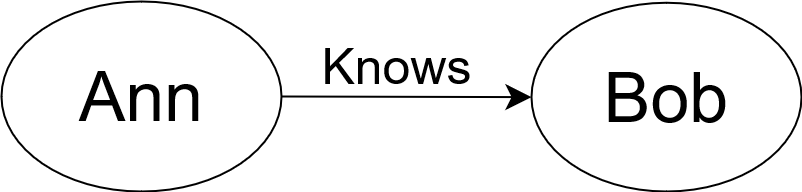
\includegraphics[scale=0.3]{figures/RDF_triple}
    \caption{TODO Informal graph of the example triples from \ref{RDF_triples_example}}
    
    \label{fig:KGexample}
\end{figure}

With this type of data organisation one can for example query for a list of all people who own cats in the dataset.

\subsection{Resource Description Framework Schema}
RDF provides the abstract model for how to organize the data and sets standards for how data points relate to eachother and real-world entities. The RDF Schema (RDFS), on the other hand, is a \emph{vocabulary} in RDF that explains how nodes of a graph relate.

\section{Semantic Triples in Description Logics}
Semantic triples are 
\fi
